\section{Confusion Matrix}
\label{confusion_matrix}

Section [REF] introduced two simple classification techniques; K-Nearest Neighbors and logistic regression.
More often than not we want to be able to quantify the performace of a classifier.
This section introduces various metrics one can do so.

\subsection{Confusion Matrix}
\label{confusion_matrix}


\begin{framed}
\begin{acknowledgement}

The following section is largely taken from \url{https://www.dataschool.io/simple-guide-to-confusion-matrix-terminology/}.
\end{acknowledgement}
\end{framed}

The confusion matrix is a popular technique to assess the quality of classifier.
In very simple words the confusion matrix is a square matrix that is used to describe the
performance of a classification model on a set of test data for which the correct classification
is known. 

Let's start exploring what a consusion matrix can tell us by considering a binary classifier.
The following table shows an assumed classifier. Here is what we can immediately infer from that matrix.

\begin{figure}[!htb]
	\begin{center}
		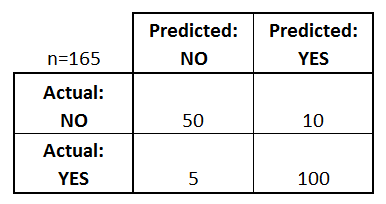
\includegraphics[scale=0.480]{imgs/confusion_matrix_simple2.png}
	\end{center}
	\caption{Binary classifier encoded into a confusion matrix. Image from \url{https://www.dataschool.io/simple-guide-to-confusion-matrix-terminology/}}
	\label{confusion_matrix_simple2. }
\end{figure}



\begin{itemize}
\item Overall we have 165 items in the data set.
\item There are two possible classes (binary classification) namely Yes and No.
\item The classifier predicted Yes 110 times and No 55 times.
\item In reality 60 items are under the class No and 105 under the class Yes.
\end{itemize}

Let'now define some basic terminology that is used when we consider a confusion matrix.


\begin{itemize}
\item True Positives or TP: The classifier predicts Yes and the are indeed classed as Yes
\item True Negatives or TN: The classifier predicts No and they are indeed classed as No
\item False Positives or FP: The classifier predicts Yes and but they are  classed as No. This is also known as Type I error
\item False Negatives or FN: The classifier predicts No but they are actually classes as Yes. This is also known as Type II error.
\end{itemize} 

\begin{framed}
\begin{remark}

All the terms defined above, are whole numbers and not rates.
\end{remark}
\end{framed}

Given this terminology here is how we could rewrite the confusion matrix as shown below

\begin{figure}[!htb]
	\begin{center}
		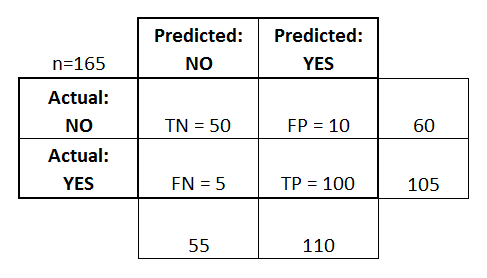
\includegraphics[scale=0.480]{imgs/confusion_matrix2.png}
	\end{center}
	\caption{Binary classifier encoded into a confusion matrix. Image from \url{https://www.dataschool.io/simple-guide-to-confusion-matrix-terminology/}}
	\label{confusion_matrix2}
\end{figure}


The confusion matrix can be used to compute various rates. The most common ones are

\begin{itemize}
\item Accuracy: overall it tells us how often is the classifier correct
\begin{equation}
\text{Accuracy} = \frac{TP + TN}{\text{total}} = \frac{100 + 50}{165} = 0.91
\end{equation}
\item Misclassification rate: overall how often is it wrong. This is also known as the error rate.
\begin{equation}
\text{Misclassification rate} = \frac{FP + FN}{\text{total}} = \frac{10 + 5}{165} = 0.09
\end{equation}
\item True Positive Rate: When it's actually yes, how often does it predict yes? This is also known as sensitivity or recall
\begin{equation}
\text{True Positive Rate} = \frac{TP}{\text{actual Yes}} = \frac{100}{105} = 0.95
\end{equation}
\item False Positive Rate: When it's actually no, how often does it predict yes? 
\begin{equation}
\text{False Positive Rate} = \frac{FP}{\text{actual No}}= \frac{10}{60} = 0.17
\end{equation}
\item True Negative Rate: When it's actually no, how often does it predict no? This is also known as specificity
\begin{equation}
\text{True Negative Rate} = \frac{TN}{\text{actual No}} = \frac{50}{60} = 0.83
\end{equation}
\item Precision: When it predicts Yes how often is it correct?
\begin{equation}
\text{Precision} = \frac{TP}{\text{Predicted Yes}} = \frac{100}{110} = 0.91
\end{equation}
\item Prevalence: How often does the yes condition actually occur in our sample?
\begin{equation}
\text{Prevalence} = \frac{\text{actual Yes}}{\text{total}} = \frac{105}{165} = 0.64
\end{equation}
\end{itemize}

There are other terms worth mentioning but we won't do that here. Instead have a look at 
the following article \url{https://www.dataschool.io/simple-guide-to-confusion-matrix-terminology/}.

\subsection{Using the \mintinline{c++}{ConfusionMatrix} class in \mintinline{c++}{jstat}}

Let's see how we can represent the example above in \mintinline{c++}{jstat}.
\mintinline{c++}{jstat} has a \mintinline{c++}{ConfusionMatrix} that is meant to model
the notion of a confusion matrix. The implementation is not restricted to binary classification.
Because of this however, the API exposed does not match the terminology above. 


\begin{minted}{c++}
package examples.ml.example8;

import maths.ConfusionMatrix;
import java.util.ArrayList;
import java.util.List;

public class Example8 {

    public static void main(String[] args){

     final int SIZE = 165;
     final int N_CLASSES = 2;

     List<Integer> actual = new ArrayList<>();

     for(int i=0; i< SIZE; ++i){

        if(i < 60){
           actual.add(0);
        }
        else{
           actual.add(1);
        }
     }

     List<Integer> predicted = new ArrayList<>();

     for(int i=0; i< SIZE; ++i){

        if(i < 50){
           predicted.add(0);
        }
        else if(i>=50 && i<65){
           predicted.add(1);
        }
        else if(i>=65 && i<70){
           predicted.add(0);
        }
        else{
           predicted.add(1);
        }
      }

      ConfusionMatrix confusionMatrix = new ConfusionMatrix(actual, predicted, N_CLASSES);

      // let's compute some metrics
      System.out.println("TP: "+confusionMatrix.getClassCounts(1));
      System.out.println("TN: "+confusionMatrix.getClassCounts(0));
      System.out.println("FP: "+confusionMatrix.getClassCountsAsOtherClass(0,1));
      System.out.println("FN: "+confusionMatrix.getClassCountsAsOtherClass(1,0));
      System.out.println("Accuracy is: " + confusionMatrix.accuracy());
      System.out.println("Misclassification Rate: " + confusionMatrix.misclassificationRate());
      System.out.println("TP Rate or Recall: " + confusionMatrix.recallClass(1));
      System.out.println("TN Rate or Specificity: " + confusionMatrix.recallClass(0));
      System.out.println("False Positive Rate: " + 
                         (double)confusionMatrix.getClassCountsAsOtherClass(0,1)/60.0);
      System.out.println("Precision: " + (double)confusionMatrix.getClassCounts(1)/
                (double) (confusionMatrix.getClassCountsAsOtherClass(0,1) + 
                          confusionMatrix.getClassCounts(1)));
      System.out.println("Prevalence: " + 
                         (double)(confusionMatrix.getClassCountsAsOtherClass(1,0) +
                          confusionMatrix.getClassCounts(1))/
                          (double) confusionMatrix.totalCount());
    }
}
\end{minted}  

Running the code above you should be getting something like the following

\begin{minted}{c++}
TP: 100
TN: 50
FP: 10
FN: 5
Accuracy is: 0.9090909090909091
Misclassification Rate: 0.09090909090909094
TP Rate or Recall: 0.9523809523809523
TN Rate or Specificity: 0.8333333333333334
False Positive Rate: 0.16666666666666666
Precision: 0.9090909090909091
Prevalence: 0.6363636363636364
\end{minted}

